%%%%%%%%%%%%%%%%%%%%%%%%%%%%% Define Article %%%%%%%%%%%%%%%%%%%%%%%%%%%%%%%%%%
\documentclass{article}
%%%%%%%%%%%%%%%%%%%%%%%%%%%%%%%%%%%%%%%%%%%%%%%%%%%%%%%%%%%%%%%%%%%%%%%%%%%%%%%

%%%%%%%%%%%%%%%%%%%%%%%%%%%%% Using Packages %%%%%%%%%%%%%%%%%%%%%%%%%%%%%%%%%%
\usepackage{geometry}
\usepackage{graphicx}
\usepackage{amssymb}
\usepackage{amsmath}
\usepackage{amsthm}
\usepackage{empheq}
\usepackage{mdframed}
\usepackage{booktabs}
\usepackage{lipsum}
\usepackage{graphicx}
\usepackage{color}
\usepackage{psfrag}
\usepackage{pgfplots}
\usepackage{bm}
%%%%%%%%%%%%%%%%%%%%%%%%%%%%%%%%%%%%%%%%%%%%%%%%%%%%%%%%%%%%%%%%%%%%%%%%%%%%%%%

% Other Settings

%%%%%%%%%%%%%%%%%%%%%%%%%% Page Setting %%%%%%%%%%%%%%%%%%%%%%%%%%%%%%%%%%%%%%%
\geometry{a4paper}

%%%%%%%%%%%%%%%%%%%%%%%%%% Define some useful colors %%%%%%%%%%%%%%%%%%%%%%%%%%
\definecolor{ocre}{RGB}{243,102,25}
\definecolor{mygray}{RGB}{243,243,244}
\definecolor{deepGreen}{RGB}{26,111,0}
\definecolor{shallowGreen}{RGB}{235,255,255}
\definecolor{deepBlue}{RGB}{61,124,222}
\definecolor{shallowBlue}{RGB}{235,249,255}
%%%%%%%%%%%%%%%%%%%%%%%%%%%%%%%%%%%%%%%%%%%%%%%%%%%%%%%%%%%%%%%%%%%%%%%%%%%%%%%

%%%%%%%%%%%%%%%%%%%%%%%%%% Define an orangebox command %%%%%%%%%%%%%%%%%%%%%%%%
\newcommand\orangebox[1]{\fcolorbox{ocre}{mygray}{\hspace{1em}#1\hspace{1em}}}
%%%%%%%%%%%%%%%%%%%%%%%%%%%%%%%%%%%%%%%%%%%%%%%%%%%%%%%%%%%%%%%%%%%%%%%%%%%%%%%

%%%%%%%%%%%%%%%%%%%%%%%%%%%% English Environments %%%%%%%%%%%%%%%%%%%%%%%%%%%%%
\newtheoremstyle{mytheoremstyle}{3pt}{3pt}{\normalfont}{0cm}{\rmfamily\bfseries}{}{1em}{{\color{black}\thmname{#1}~\thmnumber{#2}}\thmnote{\,--\,#3}}
\newtheoremstyle{myproblemstyle}{1pt}{1pt}{\normalfont}{0cm}{\rmfamily\bfseries}{}{1em}{{\color{black}\thmname{#1}~\thmnumber{#2}}\thmnote{\,--\,#3}}
\theoremstyle{mytheoremstyle}
\newmdtheoremenv[linewidth=1pt,backgroundcolor=shallowGreen,linecolor=deepGreen,leftmargin=0pt,innerleftmargin=20pt,innerrightmargin=20pt,]{theorem}{Theorem}[section]
\theoremstyle{mytheoremstyle}
\newmdtheoremenv[linewidth=1pt,backgroundcolor=shallowBlue,linecolor=deepBlue,leftmargin=0pt,innerleftmargin=20pt,innerrightmargin=20pt,]{definition}{Definition}[section]
\theoremstyle{myproblemstyle}
\newmdtheoremenv[linecolor=black,leftmargin=0pt,innerleftmargin=10pt,innerrightmargin=10pt,]{problem}{Problem}[section]
%%%%%%%%%%%%%%%%%%%%%%%%%%%%%%%%%%%%%%%%%%%%%%%%%%%%%%%%%%%%%%%%%%%%%%%%%%%%%%%

%%%%%%%%%%%%%%%%%%%%%%%%%%%%%%% Plotting Settings %%%%%%%%%%%%%%%%%%%%%%%%%%%%%
\usepgfplotslibrary{colorbrewer}
\pgfplotsset{width=8cm,compat=1.9}
%%%%%%%%%%%%%%%%%%%%%%%%%%%%%%%%%%%%%%%%%%%%%%%%%%%%%%%%%%%%%%%%%%%%%%%%%%%%%%%

%%%%%%%%%%%%%%%%%%%%%%%%%%%%%%% Title & Author %%%%%%%%%%%%%%%%%%%%%%%%%%%%%%%%
\title{Problem Checkpoint 1}
\author{Alston Yam}
\date{}
\parskip=3pt
\parindent=0pt
%%%%%%%%%%%%%%%%%%%%%%%%%%%%%%%%%%%%%%%%%%%%%%%%%%%%%%%%%%%%%%%%%%%%%%%%%%%%%%%

\begin{document}
    \maketitle

    \section*{REMEMBER!}
    \begin{enumerate}
        \item Read the question \textbf{AT LEAST TWICE} before you start.
        \item After you solve each question, CHECK, CHECK, CHECK.
    \end{enumerate}

    \section*{Special Problem:}
    \begin{problem}
        How many different paths can I take from the top left corner to the bottom right corner, if I can only go right or down?
        \begin{center}
            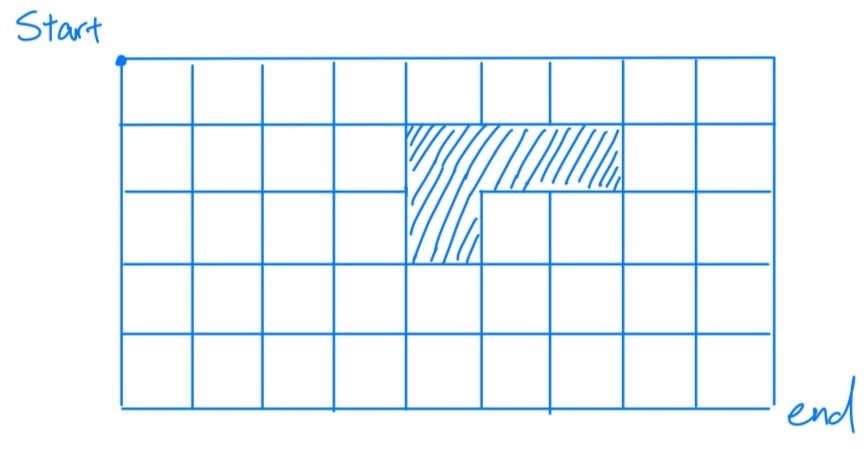
\includegraphics[width=0.6\textwidth]{checkpoint01.jpeg}
        \end{center}
    \end{problem}


    \section{Problems}
    \begin{problem}
        Make a table to show all the possible ways $\$1$ can be made using New Zealand coins. How many different ways can $\$1$ be made?
    \end{problem}

    \begin{problem}
        Louisa, Mertin, Rayman and Angela have part time jobs at Bucklands Beach VEterinary. Louisa gives the dogs baths every four days; Martin cleans out the cages in the kennels every $6$ days; Rayman feeds the animals in section two every $2$ days and Angela helps the receptionist every $3$ days. How many times in $8$ weeks will all four helpers be at Bucklands Beach Veterinary on the same day?
    \end{problem}
    
    \begin{problem}
        I roll two dice, and add up their result. What is the probability that the total I get is a multiple of $3$?
    \end{problem}

    \begin{problem}
        How many different paths can I take from the top left corner to the bottom right corner, if I can only go right or down?
        \begin{center}
            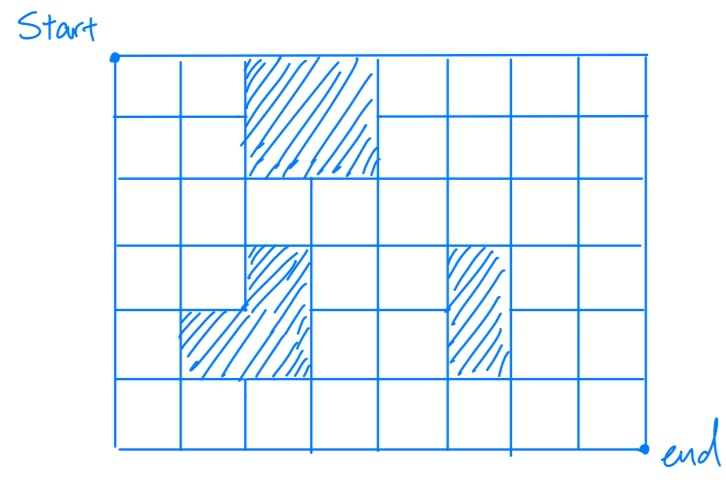
\includegraphics[width=0.6\textwidth]{checkpoint02.jpeg}
        \end{center}
    \end{problem}

    \begin{problem}
        Blake, Oliver and Vincent are building a scale model of a temple using $10$cm by $10$cm boxes. If they start with the top level of the temple being $10$cm by $20$cm (being made of $2$, $10$cm by $10$cm boxes) and the level directly below being $20$cm by $30$cm (being made of $6$, $10$cm by $10$cm boxes) and the next level being $30$cm by $40$cm; (being $12$, $10$cm by $10$cm boxes) then how many $10$cm by $10$cm boxes will they need to construct a model $10$ levels high? 
    \end{problem}

    \begin{problem}
        One year, February started and ended on the same day of the week. The $7$th of the month was a Wednesday. How many Thursdays were there in the month?
    \end{problem}

    \begin{problem}
        Alston is storing boxes of Shredded Wheat. He stores the boxes in stacks of three. Each stack is pushed up against the next stack and all the stacks sit in one long line on a shelf in his cupboard. If Alston has $36$ boxes of Shredded Wheat stacked like this, how many faces touch another face of a Shredded Wheat box?
    \end{problem}

    \begin{problem}
        Carey is trying to decide which way to go to visit her friend Isabel. There are $6$ different streets which lead to her friend's apartment building. There are three different stairways up from the street, where Carey can go into the building through two different doors. Once inside she can choose from $2$ inside stairways or $3$ elevators to get to the third floor where Isabel lives. How many different ways can carey go to visit her friend?
    \end{problem}


    
\end{document}